\documentclass[12pt,hyperref]{labbook}
\usepackage[utf8]{inputenc}
\usepackage{graphicx}
\usepackage[margin=1.0in]{geometry}
\usepackage{setspace}
\usepackage{listings}
\usepackage{color}
\usepackage{array}
\usepackage{hyperref}
\usepackage[]{algorithm}
\usepackage[noend]{algpseudocode}

\newcolumntype{P}[1]{>{\centering\arraybackslash}p{#1}}

\definecolor{dkgreen}{rgb}{0,0.6,0}
\definecolor{gray}{rgb}{0.5,0.5,0.5}
\definecolor{mauve}{rgb}{0.58,0,0.82}

\textwidth=16.5cm

\lstset{frame=tb,
  language=Java,
  aboveskip=3mm,
  belowskip=3mm,
  showstringspaces=false,
  columns=flexible,
  basicstyle={\small\ttfamily},
  numbers=none,
  numberstyle=\tiny\color{gray},
  keywordstyle=\color{blue},
  commentstyle=\color{dkgreen},
  stringstyle=\color{mauve},
  breaklines=true,
  breakatwhitespace=true,
  tabsize=3
}

\title{Notes for Undergraduate Research Work}
\author{Hollis Bui}

\begin{document}

\maketitle
\newpage
\tableofcontents
\newpage

\labday{General}

\experiment{R Notes}

Format of If/Else:

\noindent\begin{minipage}{\linewidth}
\begin{lstlisting}
if {

}else{

}
\end{lstlisting}
\end{minipage}

\experiment{TODOs}

\begin{enumerate}
    \item PANSE model implentation:
    \begin{enumerate}
        \item PANSEParameter.cpp
        \item PANSEModel.cpp
        \item PANSEParameter.h
        \item PANSEModel.h
        \item Ask about sigma term -- Done
        \item Ask about lambda prime term (is it lambda prime?) — check RFP section for how to actually calculate — DONE
    \end{enumerate}
    \item Expand Unit Testing:
    \begin{enumerate}
        \item Test Cov Matrixes — STALLED: Still need final two
        \item Test MCMC - STALLED: Need run, varyInitialConditions, calculateGewekeScore, getLogLikelihoodPosteriorMean, and setRestartFileSettings as well as two test that only functions.
        \begin{itemize}
            \item Implement other unit testing first
        \end{itemize}
        \item Parameter -- In progress
        \item Test RFP Parameter
        \item Test Trace
        \item ...Per class basis
        \item Eventually, some R scripts to do a short run for each model: Talk to Cedric
    \end{enumerate}
    \item r
    \item When working with gene-specific parameters, the openmp statements aren’t working (memory is such a mess in the area) — break down parallelization, try to find where the issue is. Perhaps start with dynamic arrays, change to vectors. Gabriel thinks the slowdown from vectors in general is made up by better parallelization in avoiding dynamic arrays.
    \begin{itemize}
        \item —STALLED. Literally can’t test speeds of various optimizations and cores right now.
    \end{itemize}
    \item Documentation
\end{enumerate}

\labday{May 13, 2016 Notes}

\experiment{PANSE Concepts}

\begin{figure}[h!]
    \center
    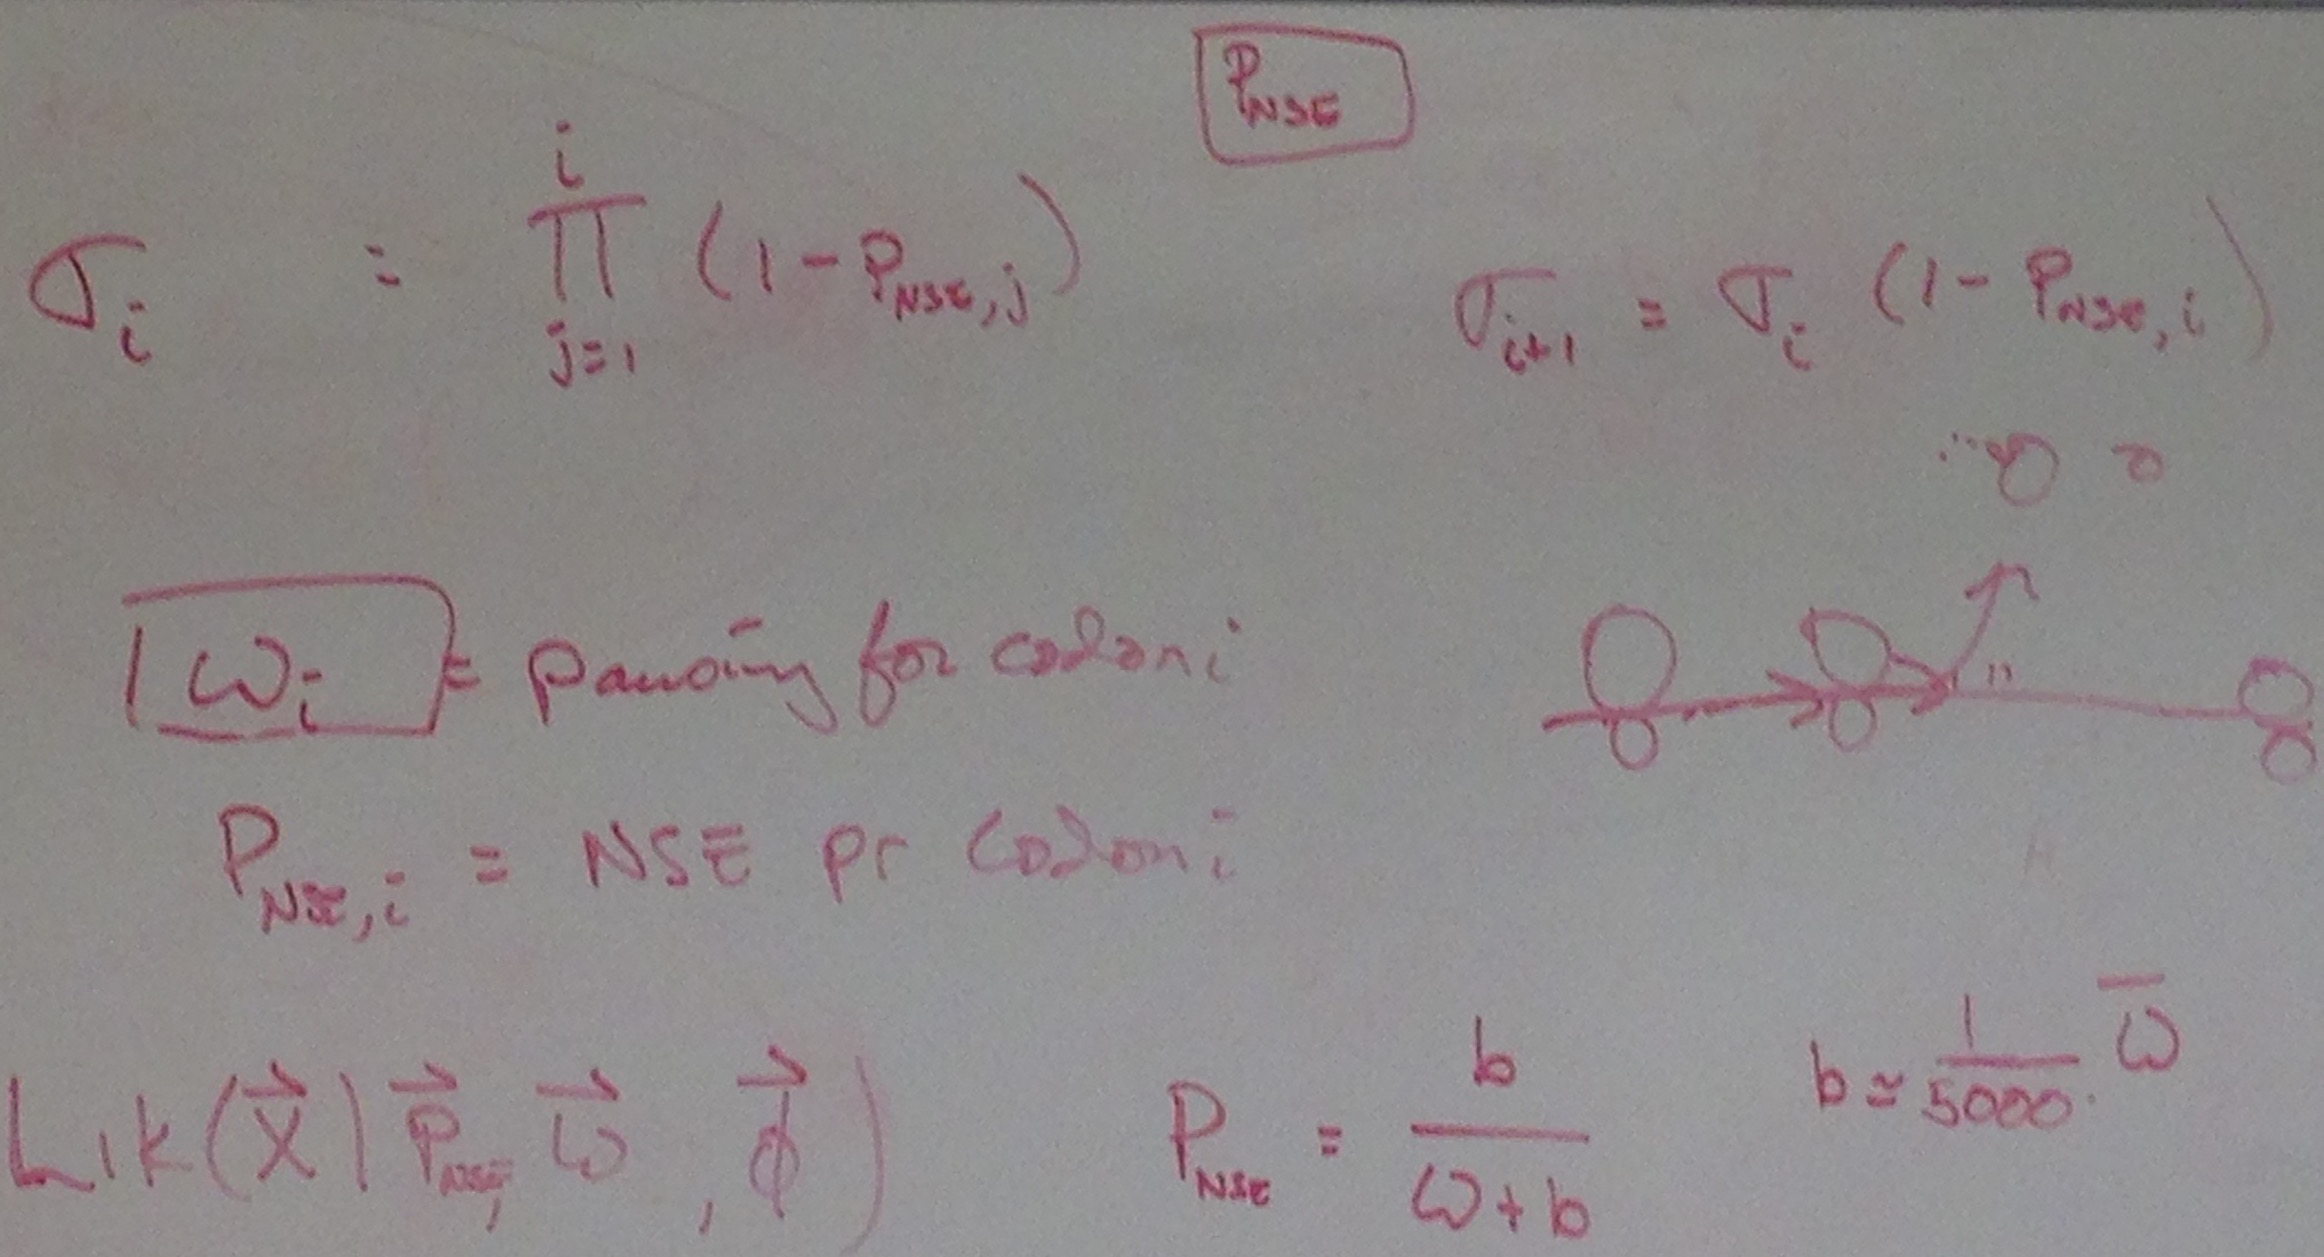
\includegraphics[width=\textwidth,keepaspectratio]{5-13-16img.jpg}
    \label{figure}
\end{figure}

\begin{equation}
    \sigma_{i} = \prod_{j=1}^{i} (1 - P_{NSE,j})
\end{equation}

$\omega_i$ = pausing for codon i

$p_nse, i$  = NSE $\Pr$ (probability) for codon i

This is codon-based.

Likelihood of the data given the parameters: 
$\mathcal{L}(\vec{x}|\vec{P_{NSE}},\vec{\omega}, \vec{\phi})$

Will be a much smaller data set, and with hundreds of calculations rather than thousands.

Randomly select $\sim$600 genes instead of 5400

Sigma vector of: $\sigma_{i + 1} = \sigma_i (1 - P_{NSE, i})$

Function is of probability of getting there vs waiting time once there

\experiment{TODOs}

\begin{itemize}
    \item Getting pausing values with simpler models (ROC)
    \item First analysis could be just estimating these terms
    \item This would mean creating a simulated data set.
    \item For simulation: $P_{NSE} = \frac{b}{\omega + b}$, where b is on the order of 1/5000 times average omega. ($b \simeq \frac{1}{5000}\overline{\omega}$) Talk to Jeremy about this, he may have finished this by now.
\end{itemize}

See the 2015 paper, 2011 paper with primal

\labday{May 19, 2016 Notes}

\experiment{PANSE Concepts}

rfp.model.pdf:
Reasoning [for lambda] is that for the sampling the Boltsman coefficient. See the explanation around equation (4) and the Z’s and Y’s.

Lambda Prime = Lambda.c * Z / Y, or call it K.

$\lambda^{\prime} = \lambda_c * \frac{Z}{Y}$

Z is the overall state space

Y is what is sampled

$\lambda_c = \lambda^{\prime} * \frac{C}{K}$. Let K be a new independent parameter, and keep track of Lambda Prime.

\labday{May 25, 2016 Notes}

\experiment{PANSE Concepts}

Codon-Specific Elongation Rate:
$P_{NSE} = \frac{b}{b + c}$ where b is where it flies off and c is where it continues.

Omega is the odds ratio of $\frac{P_{NSE}}{1 - P_{NSE}}$. Therefore $\omega = \frac{b}{c}$

Look at 2006, 2007 papers.

LOOK AT UPDATED PDF: IT’S IN FRAMEWORK

Psi (the symbol which I *thought* was Omega)
is the ribosome initiation rate: Rate at which ribosomes are jumping onto the mRA. Phi is the rate that they are jumping off at the very end.

If you have 50\% chance to get to the end, then Psi is twice as long as Phi

Phi = Psi * Sigma.

Don’t redo calculations from scratch, but rather in series.

\experiment{Parallelization}

\begin{itemize}
    \item Only 20 AA’s — Only 20 cores to spread load unto
    \item AA’s with 6 codons of course take more time than those with 2
\end{itemize}

Gilchrist thinks what is meant by Gene-Specific Parameters is to parallelize at the highest level, 
i.e. at the gene or amino acid level.

I should check the code; find where the OpenMP statements are etc

Mostly something to ask other people about if I want to tackle the problem.

\labday{May 26, 2016 Notes}

\experiment{Parallelization}

Cedric's input:
\begin{itemize}
    \item phi calculation, with mcmc accept/reject
    \item dynamic arrays
    \item big loop around everything
    \item code doesn’t work
    \item couldn’t figure out why
    \item didn’t spend that much time
\end{itemize}

we ended up parallelizing in the model class:

calculateLogLikelihoodRatioPerGene, apparently doesn’t do much.
Perhaps better to parallelize outside, with the big loop

Run a ROC model, then RFP

I’m running a fasta file that is simulated, so I know that it is true

I kinda need the R side

Get to the point where we suspect memory is the problem

Dynamic Arrays -\textgreater Vectors

\labday{May 31, 2016 Notes}

\begin{itemize}
    \item Start 1:21
    \item break 3:19
    \item back 3:24
    \item break 4:55
    \item return 5:02
    \item end 7:02
\end{itemize}

2 + 1.5 + 2

\experiment{Parallelization}

Go ahead and replace dynamic arrays with vectors, first

And then do this barebones calculation of runs to see if it makes it faster,
without regards to parallelization.

\labday{June 1, 2016 Notes}

\begin{itemize}
    \item Start 1:30
    \item Break 3:30
    \item Return 3:35
    \item End 7:00
\end{itemize}

2 + 3.5

\experiment{Parallelization}

From yesterday:

\noindent\begin{minipage}{\linewidth}
\begin{lstlisting}
0.00621732 - 10
0.00687881 - 100
0.00947537 - 1000
0.00713974 - 10000
0.00785908 - 10000
0.00750889 - 10
\end{lstlisting}
\end{minipage}

For today:

\noindent\begin{minipage}{\linewidth}
\begin{lstlisting}
0.0572747 - 10
0.0698414 - 100
\end{lstlisting}
\end{minipage}

…Odd, 10x as long on average

The above was in DEBUG mode. Release mode redos:

\begin{table}[H]
    \centering
    \begin{tabular}{|c|c|c|c|}
        \hline
        \textbf{A or V} & \textbf{Runs} & \textbf{Modifiers} & \textbf{Avg Time} \\
        \hline
        V & 100 & & 0.0141421 \\
        A & 100 & & 0.0047742 \\
        V & 10000 & & 0.00850093 \\
        A & 10000 & & 0.00479609 \\
        V & 10000 & No Deletion & 0.00871843 \\
        A & 10000 & No Deletion & 0.00491614 \\
        V & 10000 & std::sort & 0.00841396 \\
        \hline
        A & 10000 & & 0.00598796 \\
        A & 10000 & & 0.00520682 \\
        A & 100000 & & 0.00455916 \\
        A & 100000 & std::sort & 0.00776886 \\
        V & 100000 & & 0.00795495 \\
        V & 100000 & std::sort & 0.00785736 \\
        \hline
        A & 100000 & std::sort & 0.00383634 \\
        A & 100000 & & 0.00385638 \\
        A & 100000 & std::sort & 0.00392021 \\
        \hline
    \end{tabular}
\end{table}

Note: Vectors are ~2x as long on average now

\experiment{PANSE Implementation}

Next step: Make a list of everything PANSE touches and unit test these things (first and foremost before actually writing PANSE)

ALSO: Estimate and track how long, in reality, it takes to do each unit testing

PARFP, PTRFP? Just calling it RFP might be misleading.

\labday{June 2, 2016 Notes}

\begin{itemize}
    \item Start 1:01
    \item Break 3:35
    \item Return 3:50
    \item End 6:58
\end{itemize}

Spent till 4 (3 hours) compiling notes and creating a git directory.

\experiment{PANSE Implementation}

Expecting to spend ~1 hour deciding on what PANSE will need (or, rather, what RFP will need).

Talk with Gilchrist:

So data position feeds into:
\begin{itemize}
    \item a) data on gene 
    \begin{itemize}
        \item ab) to feed into ROC-RFP
    \end{itemize}
    \item or b) PANSE-RFP
\end{itemize}

\experiment{Lareau Data}
Which file type should I be reading in? RFP or Fasta?

For sample data for PANSE:

Lareau Paper -\textgreater GSE -\textgreater The untreated replicates 1,2,3. Take one, and even then only a subset of 
one of them as sample data.

The Lareau material may have undergone more processing that the new Weinberg GSE published Feb 10 2016. 

"Start with Lareau paper data" -- Gilchrist, 5:33

\labday{June 3, 2016 Notes}

\begin{itemize}
    \item Start 1:35
    \item Break 4:09
    \item Return 4:14 
\end{itemize}

\experiment{Lareau Data}

Decided to start reading the Lareau material. Began by looking directly at definition of data set
(I chose untreated replicate 1) and then parse the data to get a smaller subset (file size otherwise
is too large at 35MB)

Took longer than expected... When files finally parsed, 5:45.

Now have a data set of size 400 KB: those genes with 11 to 100 (inclusive) codons. 

\labday{June 6, 2016 Notes}

\experiment{TODOs}

Immediate future goals:
\begin{enumerate}
    \item Generate new Lareau material following specifications of Gilchrist talk, below.
    \item Just work, from now on, with the labbook class. Don't have to reformat old content.
    \item Formally write up a list of things TODO with Unit Testing for Parameter
    \item Unit Test up-to-date with Parameter
    \item Write up pseudo-code with PANSE itself to prepare for it
    \item Create and test a function for reading in Lareau material (low priority)
    \item Parallelization is after the initial PANSE stuff is implemented, very low priority
\end{enumerate}

\experiment{Lareau Data}

Talk with Gilchrist:

Let's get a randomly distributed set of data rather straight up isolation.

See below for how to randomly distribute; want only 100 genes.

61 Parameters Pausing Time

Lots of gene-specific parameters that scale with each gene.

Let's say average of each gene is ~300 AAs.

So ~7 observations per gene.

Try to get 2 parameters for a fair amount of information. Calculating at sigma is going increase at
gene length.

And of course longer gene sequences take longer to parse.

So probably want a data base for playing around with of 100 genes, between 200 and 400 AAs long

Do we need to test with all 61 parameters?
2-codon AA's are the quickest thing to work with. 

So may want to start with 100 genes of 200-400 AAs
Estimate these parameters with a small subset of the codons, starting with the 2-codon ones.
If they are behaving properly, scale up to 3/4/etc.

\noindent\makebox[\linewidth]{\rule{\paperwidth}{0.4pt}}

Long is de-facto standard
Lareau argues that Short is also relevant despite usually being thrown out

Long and short: tell how elongation is at each position.
Our model is based on pausing. 

So how do long and short factor in? Well, we don't know yet.

We could base it on just one or the other or combine the two.

For now let's just base it on Long.

\noindent\makebox[\linewidth]{\rule{\paperwidth}{0.4pt}}

After about thirty minutes following the talk with Gilchrist -- new 
subset of data produced via modifying old Perl scripts. Now have the specified data set
in the final "finalData.txt" -- 516 KB.

Interestingly small size -- seems like old data set had that many genes of smaller AA length.

\noindent\makebox[\linewidth]{\rule{\paperwidth}{0.4pt}}

Spent an hour afterward reading over labbook documentation and reformatting notes where needed.

\labday{June 7, 2016 Notes}
In the course of running an RFP Model, the following functions are called (and have yet to be
unit tested).

\begin{itemize}
    \item initParameterSet (actually already done... mostly) -- general parameter
    \begin{itemize}
        \item test std\_csp changes -- Done
        \item test numAcceptForCodonSpecificParameters changes -- Done
        \item Possibly setNumMutationSelectionValues -- Ignore for now
        \item Possibly initCategoryDefinitions --Ignore for now
        \item For the two above -- Find how to check delM and delEta of category (a vector of Mixture Definitions) -- Done
        \item Check many final changes at the end of this function -- Three remaining
    \end{itemize}
    \item initRFPParameterSet -- RFP exclusive
    \item getSelectionCategory -- general parameter
    \item InitializeSynthesisRate -- general parameter
    \begin{itemize}
        \item calculateSCUO
        \item quickSortPair
        \item quickSort
        \item Parameter::randLogNorm
    \end{itemize}
    \item setParameter -- RFP model exclusive
    \item mcmc.run -- MCMC function on RFP(TODO later?)
\end{itemize}

Going to take it one step at a time, finish up initParameterSet testing...

Finished most of initParameterSet completely. Need to ask Cedric about a duplicate function before
finishing the final two functions.

May need to write a function to unit test with the categories variable itself, but
all that happens otherwise is it pushes unto the vector of vector of vectors.

Encountering a strange printing bug right before the end. While if statement works correctly,
the final confirmation of initParameterSet isn't being printed.

Example output:


\noindent\begin{minipage}{\linewidth}
\begin{lstlisting}
Parameter getMixtureAssignment --- Pass
Parameter setMixtureAssignment --- Pass
Parameter getMutationSelectionState --- Pass
Parameter getNumParam --- Pass
Parameter getNumMixtureElements --- Pass
Parameter getStdDevSynthesisRate --- Pass
Parameter setStdDevSynthesisRate --- Pass
Parameter getCurrentStdDevSynthesisRateProposalWidth --- Pass
Parameter getNumAcceptForStdDevSynthesisRate --- Pass
Parameter getStdCspForIndex --- Pass
Parameter getNumAcceptForCspForIndex --- Pass
Parameter getNumMutationCategories --- Pass
Parameter getNumSelectionCategories --- Pass
Parameter getMutationCategory --- Pass
Parameter getSelectionCategory --- Pass
Parameter getMixtureElementsOfMutationCategory --- Pass
Parameter getMixtureElementsOfSelectionCategory --- Pass
Parameter getCategoryProbability --- Pass
Parameter setCategoryProbability --- Pass
Parameter getSynthesisRate --- Pass
Parameter setSynthesisRate --- Pass
Parameter getSynthesisRateProposalWidth --- Pass
0
Parameter initParameterSet --- Pass

Process finished with exit code 0
\end{lstlisting}
\end{minipage}

vs

\noindent\begin{minipage}{\linewidth}
\begin{lstlisting}
Parameter getMixtureAssignment --- Pass
Parameter setMixtureAssignment --- Pass
Parameter getMutationSelectionState --- Pass
Parameter getNumParam --- Pass
Parameter getNumMixtureElements --- Pass
Parameter getStdDevSynthesisRate --- Pass
Parameter setStdDevSynthesisRate --- Pass
Parameter getCurrentStdDevSynthesisRateProposalWidth --- Pass
Parameter getNumAcceptForStdDevSynthesisRate --- Pass
Parameter getStdCspForIndex --- Pass
Parameter getNumAcceptForCspForIndex --- Pass
Parameter getNumMutationCategories --- Pass
Parameter getNumSelectionCategories --- Pass
Parameter getMutationCategory --- Pass
Parameter getSelectionCategory --- Pass
Parameter getMixtureElementsOfMutationCategory --- Pass
Parameter getMixtureElementsOfSelectionCategory --- Pass
Parameter getCategoryProbability --- Pass
Parameter setCategoryProbability --- Pass
Parameter getSynthesisRate --- Pass
Parameter setSynthesisRate --- Pass
Parameter getSynthesisRateProposalWidth --- Pass


Process finished with exit code 0
\end{lstlisting}
\end{minipage}

\end{document}
